\chapter{Validación del algoritmo de visión artificial}


\section{Metodología}
En esta sección se describe el procedimiento realizado para llevar a cabo la adecuación del algoritmo de visión artificial para la detección de compuertas dentro del circuito de vuelo. Cabe mencionar que, como se mostró en la sección anterior, el tipo de compuertas seleccionadas para la formación del circuito de vuelo fue un modelo similar al utilizado en las competencias del IROS, con un característico color naranja. Ahora bien, debido a que el algoritmo de visión artificial está basado en la detección de color el aspecto más importante para adecuar el algoritmo es encontrar el rango de color, en la escala HSV, adecuado para nuestro objeto; es decir, sintonizar los parámetros del modelo de color para el color naranja.

Entonces, para lograr sintonizar lo mejor posible la escala de color, se utilizó como base un rango de color adecuado para detectar el color naranja, pues este es el color principal del objeto de interés; sin embargo, el color de las compuertas es una de la infinidad de tonalidades derivadas del naranja, por lo que fue necesario ajustar más el rango para que, de ser posible, el algoritmo fuera capaz de detectar exclusivamente las compuertas y no diera falsos positivos con objetos con una tonalidad derivada del naranja. Por otro lado, dentro del circuito de vuelo el único objeto con una tonalidad similar al color naranja es el edificio rojo que se encuentra detrás de la primera compuerta, por lo que, se están asumiendo condiciones prácticamente ideales para la detección de las compuertas.

Dicho lo anterior, la figura \ref{fig:cv_hsv} corresponde al mapa de color utilizado para definir el rango base para el algoritmo de detección. El diagrama está compuesto por 3 partes: el eje \textit{x} corresponde al rango de tonos para el matiz (hue); la primera parte del eje \textit{y}, denotada con un (1), pertenece a los tonos de matiz con una saturación que varía entre 0 y 255. Por último, la segunda parte del eje \textit{y}, identificada con un (2), denota los tonos de matiz para los cuales los coeficientes de saturación y valor son iguales a 255. 

Entonces, para obtener la escala para la detección de un color, se debe escoger el tono de matiz y saturación correspondiente, y posteriormente establecer el coeficiente de valor entre 25 y 255.

Por lo tanto, a partir de la figura \ref{fig:cv_hsv} la escala base seleccionada para la detección del color naranja fue: \[H:5-25;\text{ } S:75-255;\text{ } V:25-255\]

\begin{figure}[ht]
    \centering
    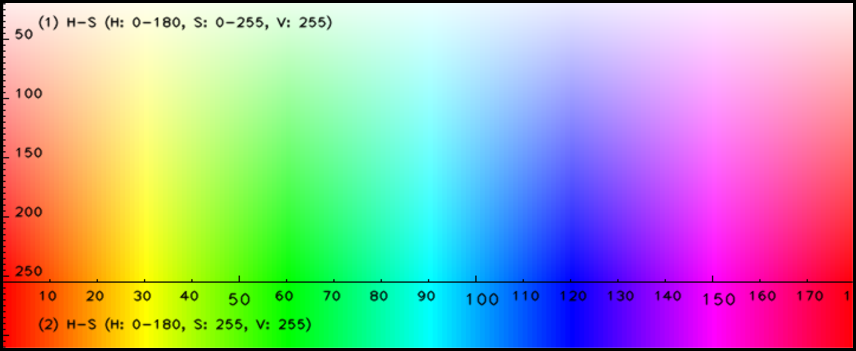
\includegraphics[width=0.8\textwidth]{cv_hsv.pdf}
    \caption{Mapa de color en escala HSV \cite{dey_2020}}
    \label{fig:cv_hsv}
\end{figure}

\section{Sintonización de la escala de color}

La sub-sección anterior representa el argumento para la selección de la escala inicial, ahora bien, como se mencionó al inicio de esta sección, fue necesario ajustar el rango de color para proveer al algoritmo de mayor precisión y robustez al momento de detectar las compuertas del circuito de vuelo. Lo anterior se logró utilizando imágenes del ambiente de simulación, de tal manera que se aplicó una máscara con el rango de color especificado y se fueron variando los valores de las componentes del modelo de color hasta observar que el algoritmo aislaba de manera satisfactoria las compuertas del resto de objetos en el circuito. 

La figura \ref{fig:cv_gates} muestra las imágenes utilizadas con este fin. La figura \ref{fig:cv_gate1} corresponde a una fotografía obtenida a partir de la cámara simulada a bordo del dron, se trata de un primer plano hecho a una de las compuertas del circuito de vuelo; además, la figura \ref{fig:cv_gate2} corresponde a una toma captada en tercera persona, en donde hay dos compuertas visibles y el dron intenta cruzar a través de una de ellas, incluso puede notarse el fotograma captado por la cámara del dron. Por otro lado, la figura \ref{fig:cv_gate3} presenta otra toma en tercera persona, en donde es visible una compuerta y el dron se encuentra estático en el suelo, en este caso es posible destacar el uso de un ambiente diferente al ambiente utilizado en el circuito de vuelo final. Por último, la figura \ref{fig:cv_gate4} presenta una toma del circuito de vuelo en donde se alzan a apreciar dos compuertas y el único edificio incluido en el ambiente de simulación. 

Cabe destacar que  con las figuras \ref{fig:cv_gate3} y \ref{fig:cv_gate4} se buscó darle mayor robustez al algoritmo de detección de compuertas, utilizando otro tipo de ambiente y objetos de otros colores para realizar una calibración más adecuada del rango de color utilizado.

A partir de lo ya mencionado, para realizar la sintonización del rango de color se elaboró un script de Python, en donde se hizo uso de OpenCV para cargar las imágenes mostradas en la figura \ref{fig:cv_gates}, convertir su modelo de color de BGR a HSV, y posteriormente ejecutar el algoritmo de detección con la escala de color base. Lo anterior se realizó de manera individual con cada una de las imágenes, de tal manera que con cada una se ajustó la escala base de forma gradual hasta observar una detección aceptable; es decir, hasta que la detección eliminara la mayor cantidad de falsos positivos en la imagen, dejando solamente las siluetas de las compuertas. 

Es importante mencionar que en este punto del desarrollo del trabajo, el algoritmo no se encontraba ejecutándose de forma indefinida en algún proceso, sino que, se ejecuta una sola vez sobre cada imagen, por lo que lo único que se necesitó para realizar la sintonización fueron las imágenes mencionadas para realizar el ajuste; es decir, el script elaborado no requiere de la ejecución del ambiente creado en Gazebo o de una instancia del SITL de ArduPilot para realizar el ajuste de la escala, este funciona de forma independiente y permite ajustar los parámetros del modelo de color de forma dinámica. El proceso seguido para ejecutar el algoritmo desde un nodo en ROS se describe más adelante, en su respectiva sección.


\begin{figure}[ht]
    \centering
    \subfloat[]{\label{fig:cv_gate1}{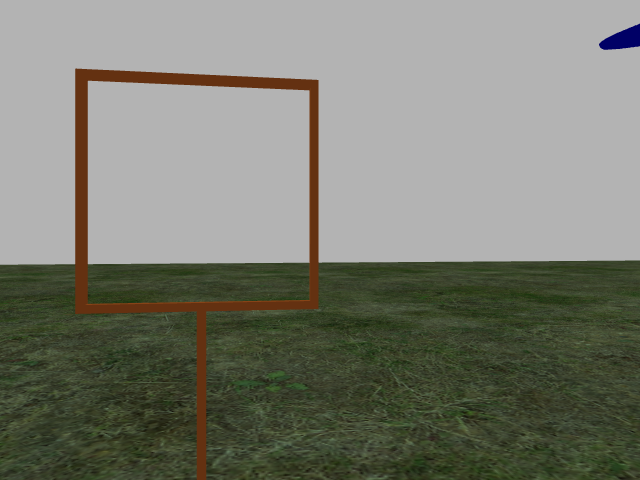
\includegraphics[width=0.48\textwidth]{Gate.png}}}\hfill
    \subfloat[]{\label{fig:cv_gate2}{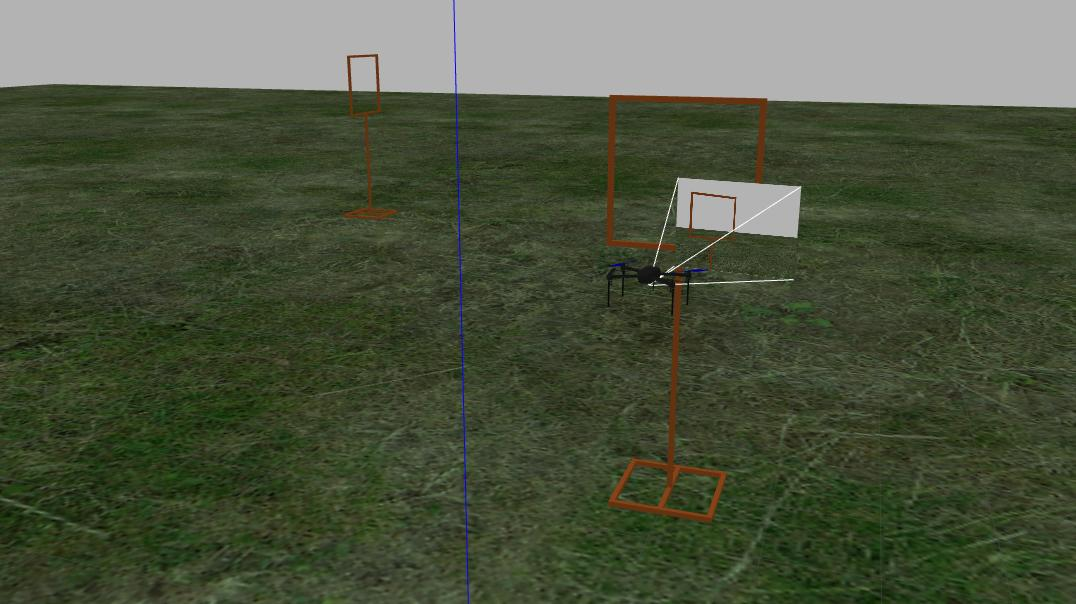
\includegraphics[width=0.48\textwidth]{Gate2.jpg}}}\\
    \subfloat[]{\label{fig:cv_gate3}{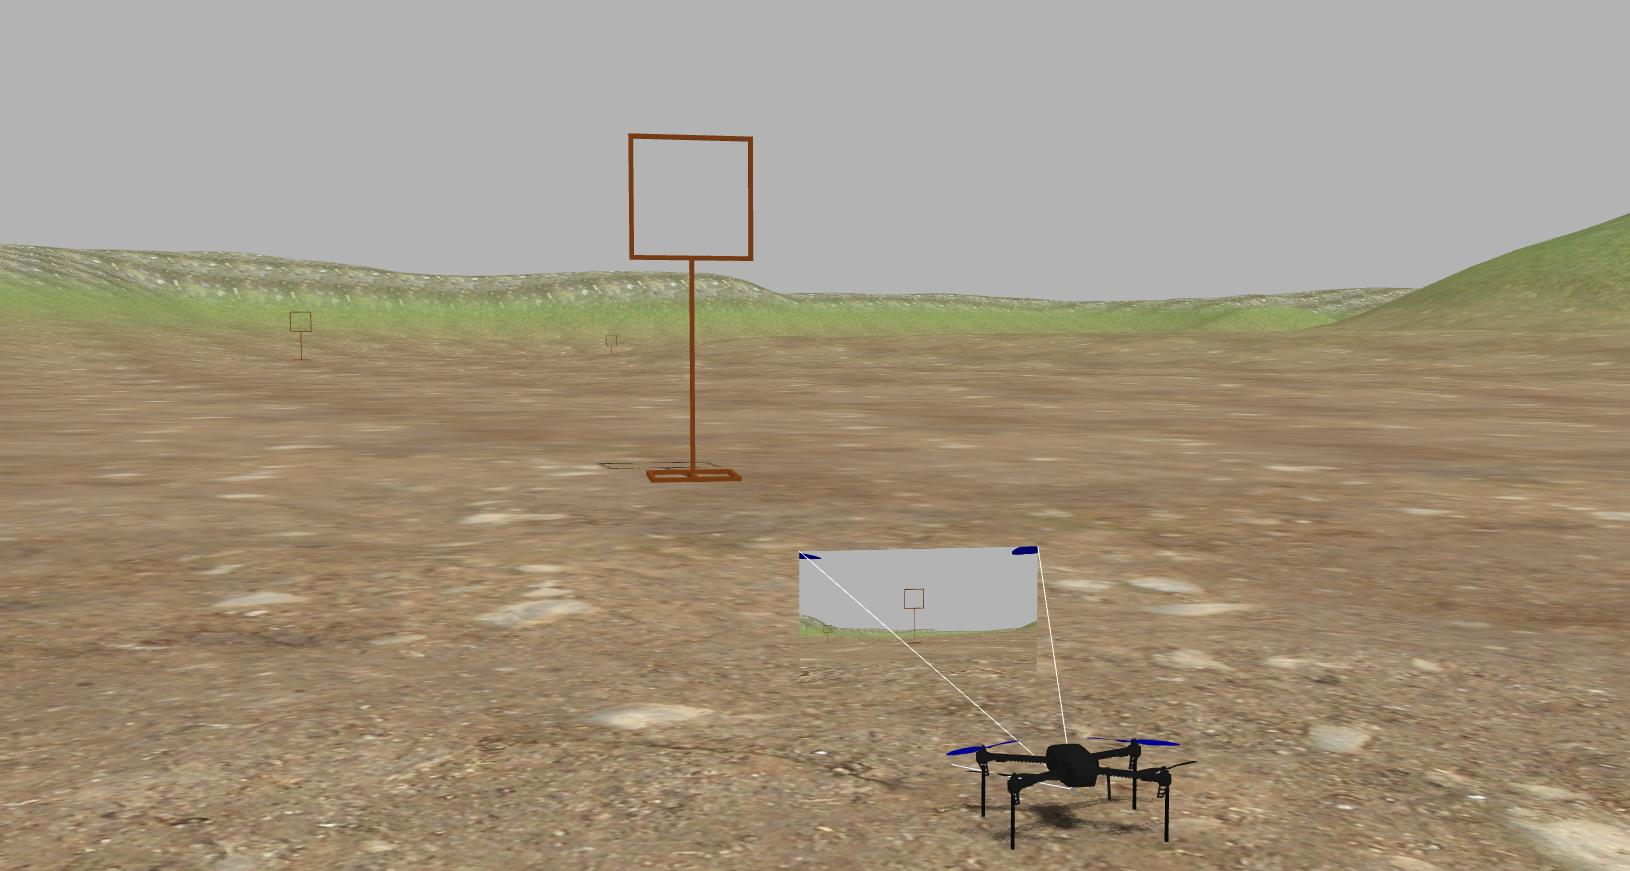
\includegraphics[width=0.48\textwidth]{Gate3.jpg}}}\hfill
    \subfloat[]{\label{fig:cv_gate4}{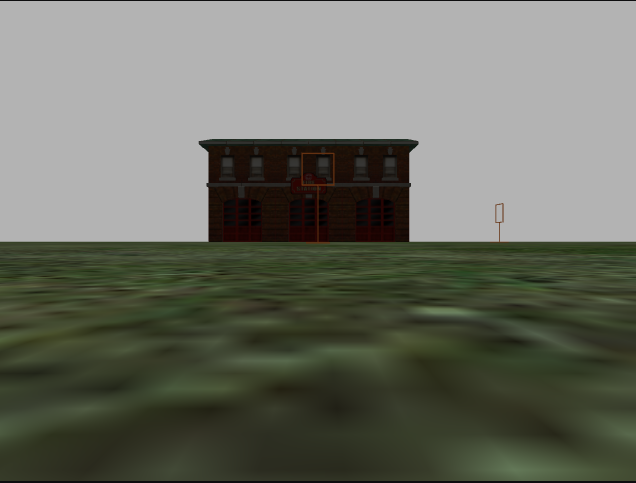
\includegraphics[width=0.48\textwidth]{Gate4.png}}}\hfill

    \caption{Imágenes utilizadas para la sintonización del rango de color}
    \label{fig:cv_gates}
\end{figure}

Entonces, a partir de la escala base se realizó la primera prueba del algoritmo de detección sobre la colección de imágenes. La figura \ref{fig:cv_gatesth1} muestra los resultados obtenidos en esta prueba. Tomando en cuenta el contexto anterior, la figura \ref{fig:cv_gate1th1} muestra la detección efectuada en la imagen en primer plano de una de las compuertas, como se puede observar, la detección es prácticamente perfecta y se logra aislar con gran precisión la compuerta del fondo, el suelo y el fragmento visible de pala de uno de los rotores del dron. Después, la figura \ref{fig:cv_gate2th1} presenta la fotografía en tercera persona de las dos compuertas, se aprecia que se logra aislar de gran manera el contorno de las compuertas, dejando a un lado el suelo y el dron;  sin embargo, el algoritmo no es capaz de detectar el fragmento de compuerta que se observa en la previsualización de la toma de la cámara del dron. Además, la figura \ref{fig:cv_gate3th1} presenta el comportamiento que se presentó sobre la imagen con cambio de ambiente, es posible observar que en este caso la detección es menos exacta, pues si bien es posible apreciar el aislamiento de gran parte del contorno de la compuerta, el suelo del ambiente también forma parte de la detección, esto se debe a que su tonalidad entra en el rango de color de la escala base. Por último, la figura \ref{fig:cv_gate4th1}, presenta el efecto de la detección sobre la imagen con el edificio del ambiente de simulación en el fondo, está último caso presenta el peor desempeño por parte del algoritmo de detección, pues no fue capaz de captar en absoluto las compuertas de la imagen, sino que, más bien aisló la fachada rojiza del edificio; estas dos últimas pruebas son un claro ejemplo del porqué fue necesario realizar ajustes en el rango de color utilizado.


\begin{figure}[ht]
    \centering
    \subfloat[]{\label{fig:cv_gate1th1}{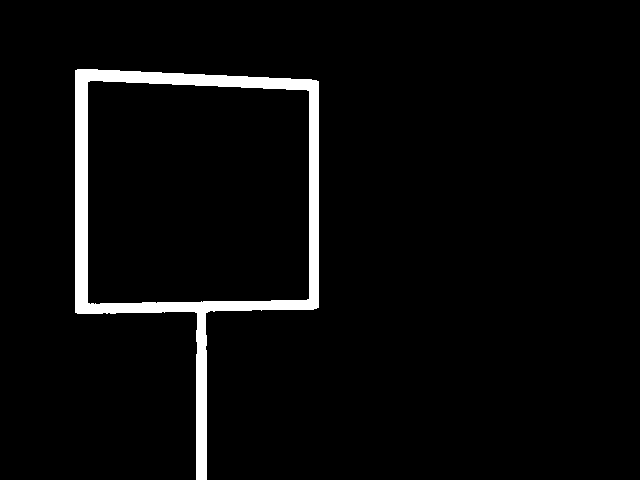
\includegraphics[width=0.48\textwidth]{Gate1_TH1.png}}}\hfill
    \subfloat[]{\label{fig:cv_gate2th1}{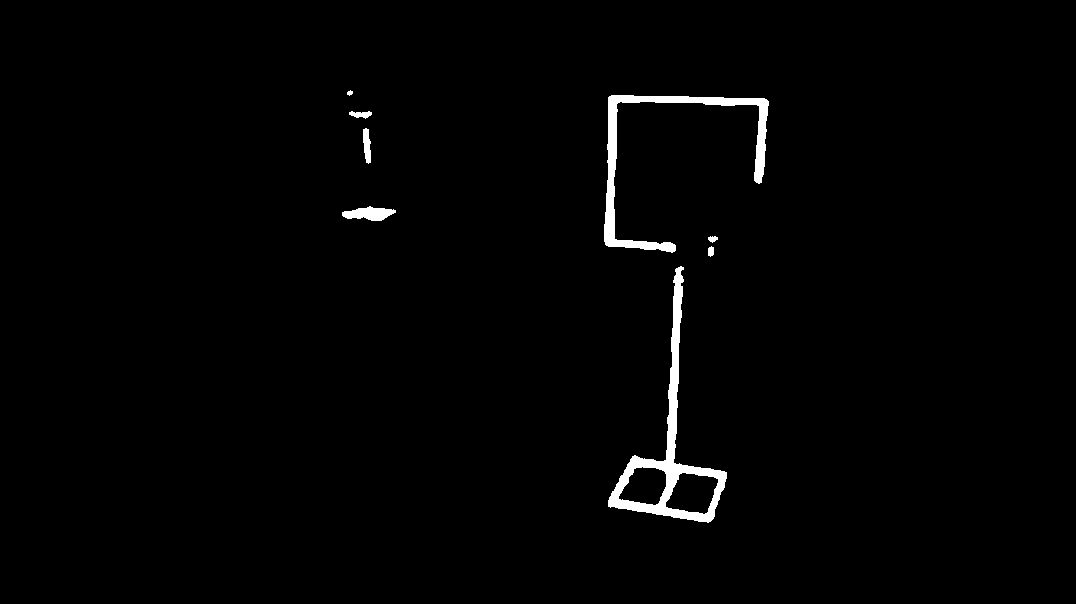
\includegraphics[width=0.48\textwidth]{Gate2_TH1.png}}}\\
    \subfloat[]{\label{fig:cv_gate3th1}{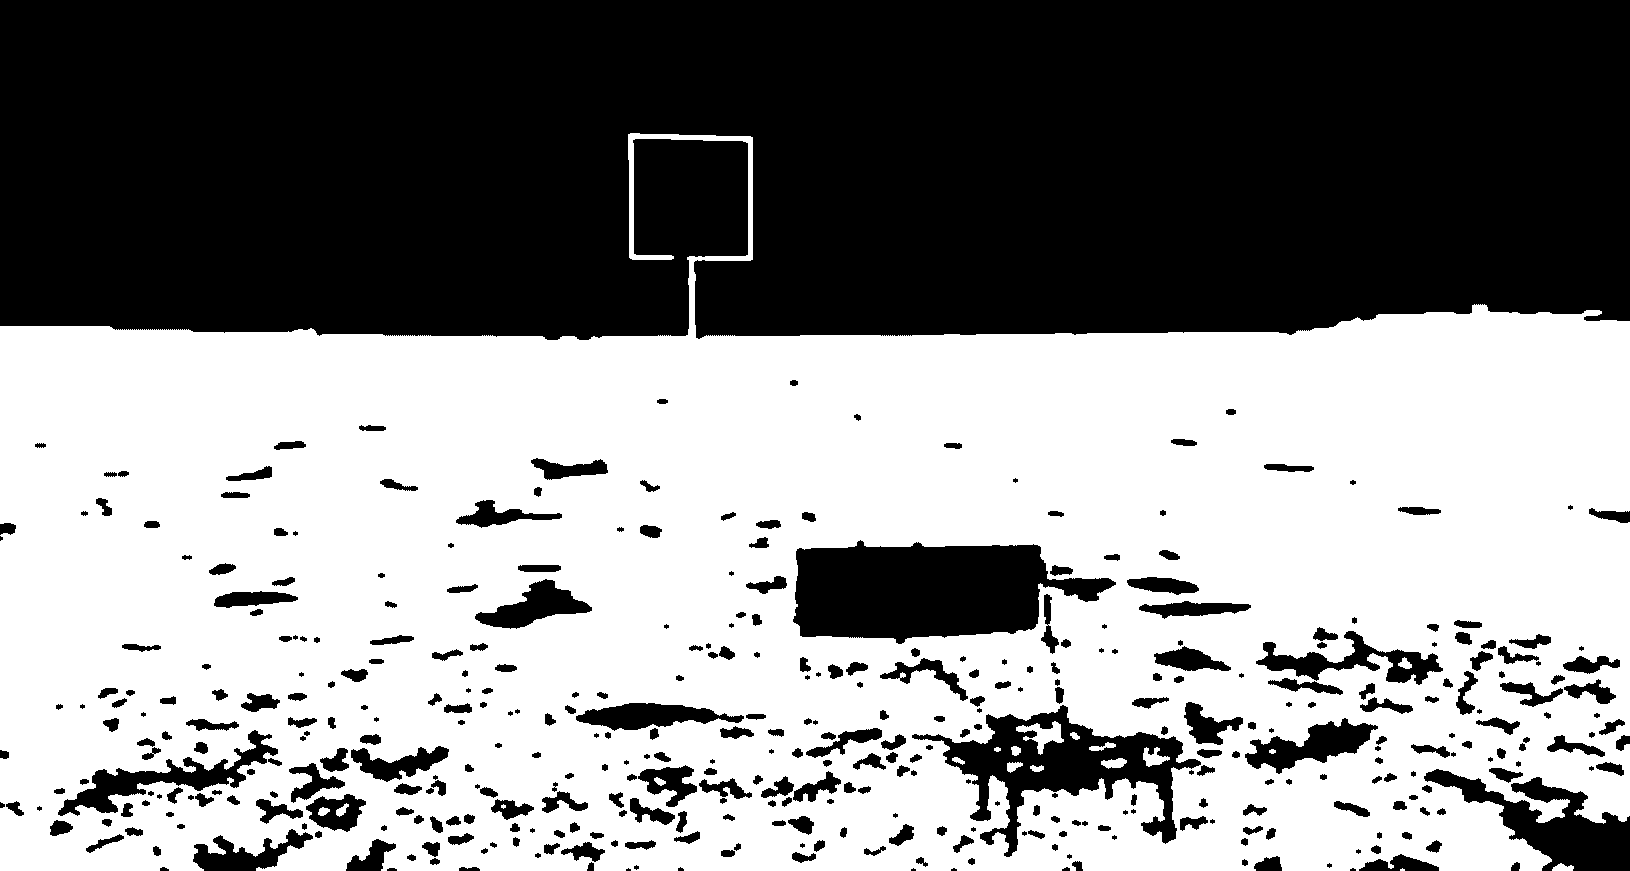
\includegraphics[width=0.48\textwidth]{Gate3_TH1.png}}}\hfill
    \subfloat[]{\label{fig:cv_gate4th1}{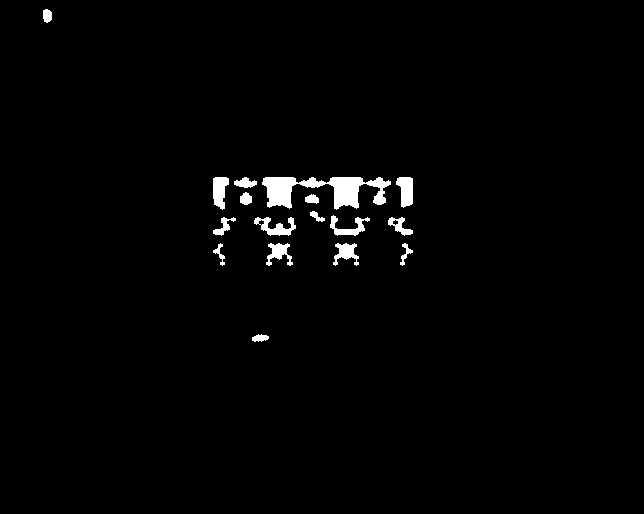
\includegraphics[width=0.48\textwidth]{Gate4_TH1.png}}}\hfill

    \caption{Detección de compuerta con el primer rango de color}
    \label{fig:cv_gatesth1}
\end{figure}

Dándole continuidad a lo observado, se continuó con el ajuste del rango base; se llegó a una serie de valores que mejoraron notablemente el desempeño del algoritmo de detección. El proceso para la sintonización fue el mismo, de tal manera que se jugó con el límite inferior de cada parámetro en el modelo de color HSV hasta que se observó una mejora en la detección de cada una de las imágenes, principalmente en las últimas dos pues son las que presentaron los resultados más paupérrimos en las primeras pruebas. Entonces, el rango de color que se obtuvo con el reajuste es el siguiente: \[H:5-25;\text{ } S:99-255;\text{ } V:77-171\]

Se observa que el rango para el matiz permaneció igual, mientras que los parámetros de saturación y valor percibieron un cambió un tanto significativo. La figura \ref{fig:cv_gatesth2} muestra los resultados obtenidos a partir de sintonización realizada, se presenta el mismo número de imágenes que en la prueba anterior, y es posible observar que la detección para la figura \ref{fig:cv_gate1th2} y \ref{fig:cv_gate2th2} permaneció prácticamente igual, aun que no del todo. Realmente el desempeño logrado en la figura \ref{fig:cv_gate1th2} fue bastante bueno, por lo que en este caso no se observa ninguna mejora en particular. Por otro lado, en cuanto a la figura \ref{fig:cv_gate2th2}, es posible observar que el reajuste provocó la eliminación de algunas secciones de la compuerta más cercana al dron, para la segunda compuerta de la imagen, se observa una perdida de área detectada bastante significativa; sin embargo, esto no representa un comportamiento no deseado, del todo, pues tomando en cuenta el objetivo del algoritmo de detección y la ruta de vuelo seguida por el dron, se puede llegar a la conclusión de que realmente en ningún momento del vuelo el dron tendrá en su campo de visión a más de una compuerta a la vez, y si lo llega a hacer, lo que se busca es que el dron sea capaz de detectar la compuerta más cercana a él, por lo que las compuertas del fondo pierden cierto grado de relevancia para esta aplicación en particular. 

En contraste con el caso anterior, el desempeño referente a la figura \ref{fig:cv_gate3th2} presenta una gran mejora con respecto a la primera prueba realizada, a tal grado que el porcentaje de falsos positivos obtenidos por la tonalidad del suelo resulta ser mucho menor, y en este caso ya es posible observar en mayor proporción el contorno y superficie de la compuerta. Por otro lado, la detección efectuada en la figura \ref{fig:cv_gate4th2} sigue siendo bastante pobre, y al realizar el reajuste de la escala de color, ya no fue posible detectar ningún objeto dentro de esta imagen, por lo que la imagen resultante se encuentra completamente en negro.


\begin{figure}[ht]
    \centering
    \subfloat[]{\label{fig:cv_gate1th2}{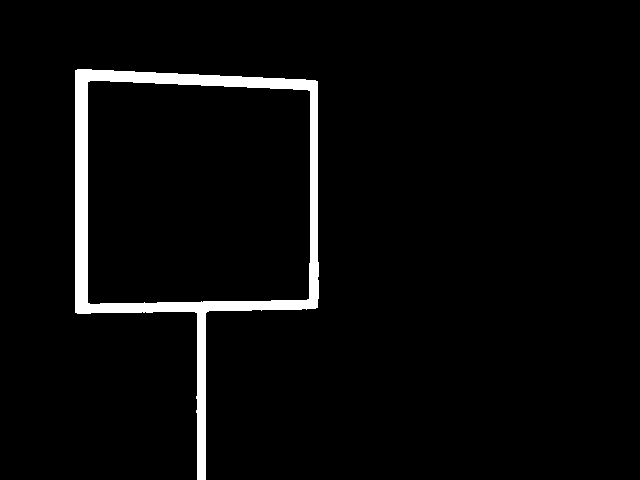
\includegraphics[width=0.48\textwidth]{Gate1_TH2.png}}}\hfill
    \subfloat[]{\label{fig:cv_gate2th2}{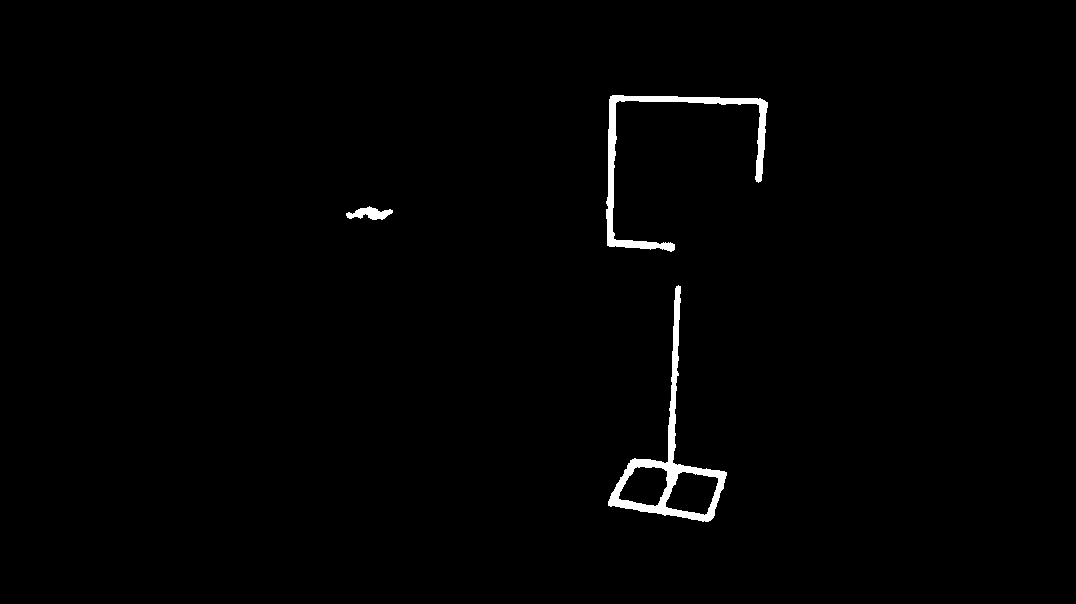
\includegraphics[width=0.48\textwidth]{Gate2_TH2.png}}}\\
    \subfloat[]{\label{fig:cv_gate3th2}{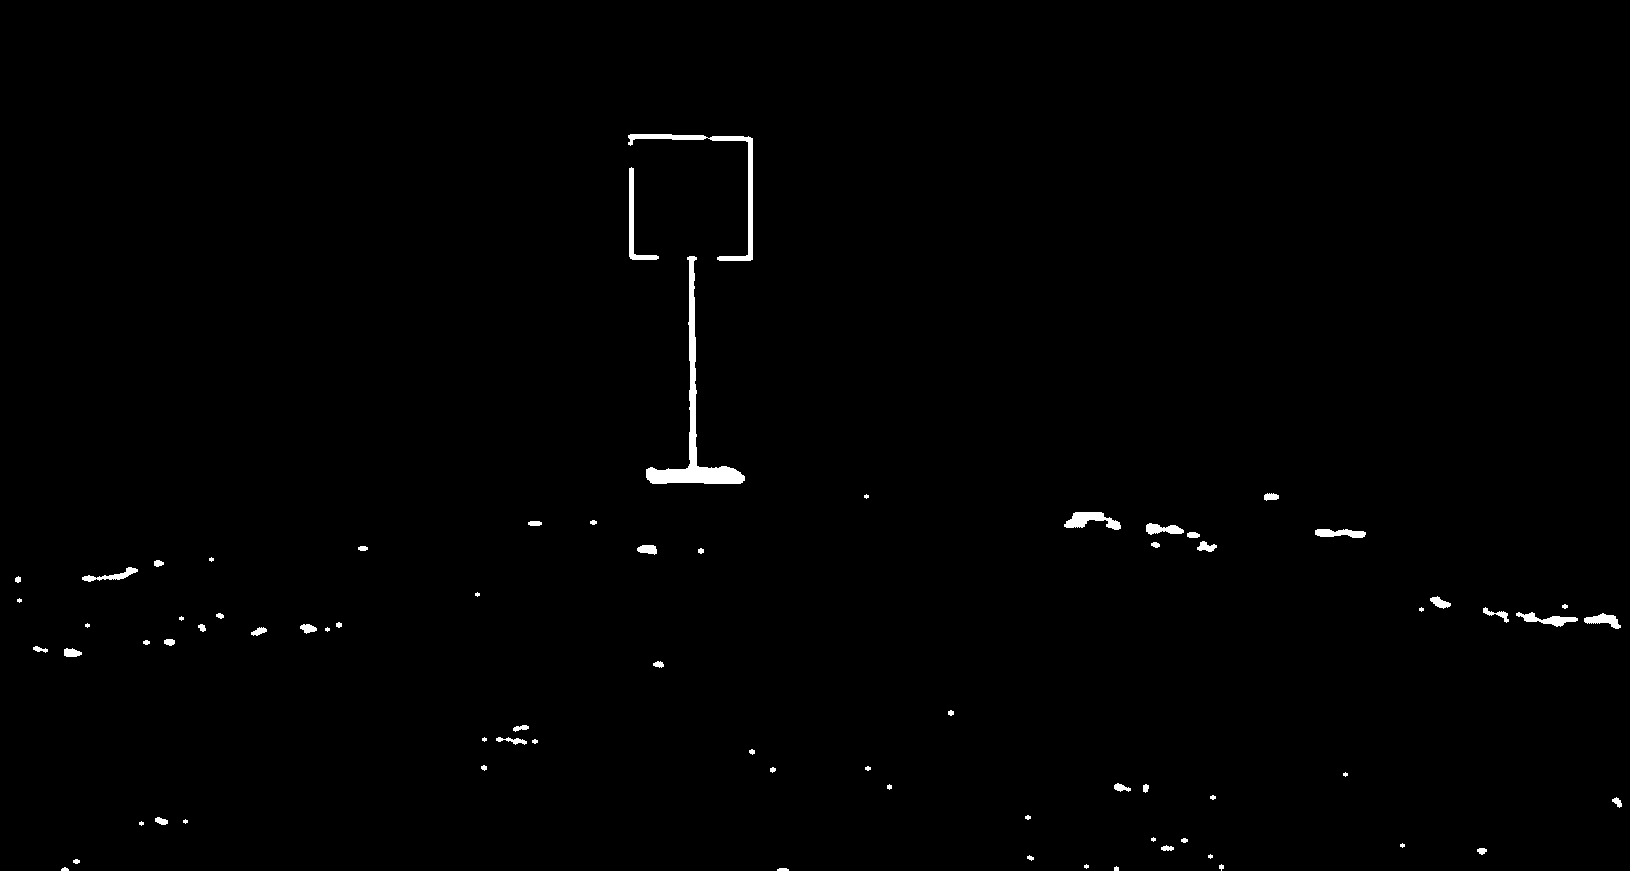
\includegraphics[width=0.48\textwidth]{Gate3_TH2.png}}}\hfill
    \subfloat[]{\label{fig:cv_gate4th2}{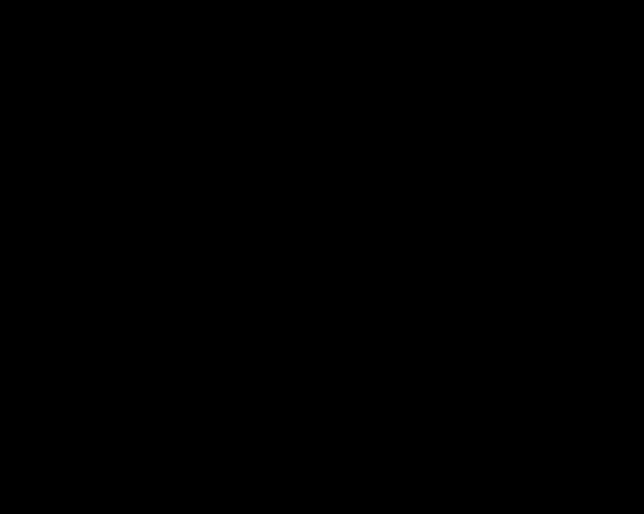
\includegraphics[width=0.48\textwidth]{Gate4_TH2.png}}}\hfill

    \caption{Sintonización del rango de color}
    \label{fig:cv_gatesth2}
\end{figure}

Recapitulando un poco lo ya comentado, el reajuste en la escala de color permitió obtener una mejora bastante significativa para la reducción de falsos positivos en la detección de las compuertas; sin embargo, contrario o lo que se esperaba, el desempeño que se obtuvo en la última imagen resulto ser inferior al de la primera prueba. Entonces, se buscó realizar una segunda sintonización con el objetivo de mejorar el desempeño en esta última imagen, por lo que ya no se realizaron más pruebas con el resto de imágenes, y el reajuste se realizó únicamente experimentando con este último fotograma. Dando como resultado el siguiente rango de parámetros:\[H:0-25;\text{ } S:45-217;\text{ } V:0-44\]

Sin embargo, este rango sigue sin presentar una detección adecuada para este último caso; es decir, pese a los esfuerzos realizados, no se logró encontrar un rango de valores que mejoraran la detección, el algoritmo no fue capaz de detectar la compuerta.

\begin{figure}[ht]
    \centering
    \subfloat[]{\label{fig:cv_gate1th3}{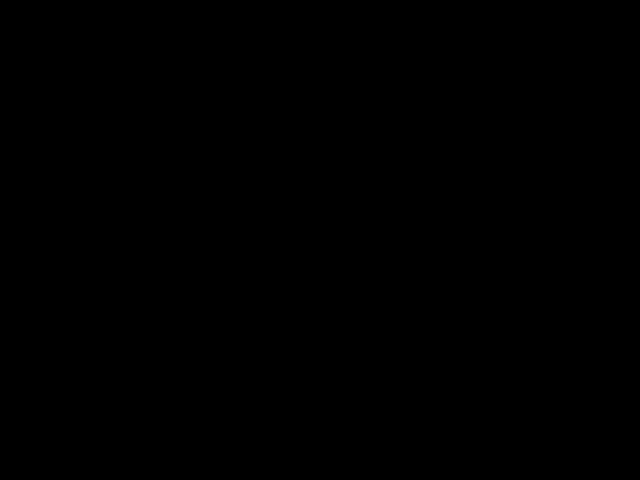
\includegraphics[width=0.48\textwidth]{Gate1_TH3.png}}}\hfill
    \subfloat[]{\label{fig:cv_gate4th3}{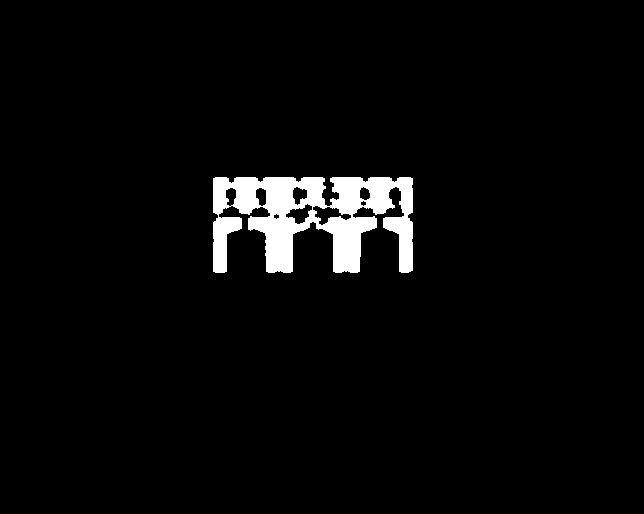
\includegraphics[width=0.48\textwidth]{Gate4_TH3.png}}}

    \caption{Intento de sintonización utilizando la cuarta imagen de referencia como base}
    \label{fig:cv_gatesth3}
\end{figure}

Lo anterior se atribuye a que, debido a la distancia con la que fue tomada la imagen, la proporción de superficie de las compuertas en la imagen es bastante reducida, por lo que el algoritmo no es capaz de aislar de manera satisfactoria el color que se busca. La figura \ref{fig:cv_gatesth3} presenta los resultados obtenidos con este último intento de resintonización. En la figura \ref{fig:cv_gate4th3} es posible observar el desempeño de la detección en la imagen objetivo, se puede apreciar que solamente fue posible mejorar el aislamiento de la fachada del edificio.

Entonces, se utilizó esta última escala de color para ejecutar la detección en el resto de fotografías, y lo que se obtuvo fue algo similar a lo observado en la figura \ref{fig:cv_gate1th3}. Esta figura corresponde solamente a la detección efectuada sobre la toma en primer plano de la compuerta; sin embargo, el resultado obtenido en las otras imágenes fue el mismo, un recuadro completamente negro.

Finalmente, está claro que este último rango de parámetros no es para nada eficiente y no cumple con el objetivo de la detección de compuertas, por lo que al final se descartó y se utilizó la escala obtenida a partir del primer ajuste para su implementación en ROS.



\section{Algoritmo de visón artificial}

En la sub-sección anterior se describió el proceso implementado para adecuar el algoritmo de detección con base en los requerimientos mencionados. Ahora, esta última sub-sección tiene como objetivo definir la lógica secuencial utilizada, así como las funciones que componen el algoritmo implementado.

La estructura de la lógica implementada puede observarse en el algoritmo \ref{alg:vision}
\begin{algorithm}
\caption{Metodología para la detección de compuertas}\label{alg:vision}
\begin{algorithmic}
\State \textbf{1. Adquirir} imagen
\State \textbf{2. Convertir }espacio de color: $\text{RGB} \to \text{BGR}$
\State \textbf{3. Convertir }espacio de color: $\text{BGR} \to \text{HSV}$
\State \textbf{4. Aplicar }el método del valor umbral sobre la imagen
\State \textbf{5. Aplicar }una operación de apertura sobre la imagen umbralizada
\State \textbf{6. Aplicar }una operación de cerradura sobre la imagen umbralizada
\State \textbf{6. Mostrar } la imagen original y la imagen procesada
\end{algorithmic}
\end{algorithm}

Como se puede observar, es un algoritmo bastante sencillo. Ahora bien, como se mencionó en el marco teórico, OpenCV ofrece una gran variedad de funciones y herramientas para la ejecución de algoritmos de visión artificial, por lo que el programa resultante es bastante compacto en cuanto a líneas de código, pues se utilizaron funciones nativas de la librería. El código desarrollado para esta etapa puede ser consultado en el repositorio oficial del presente trabajo, \citet{Axolotl}, dentro del directorio de recursos.

A continuación se describen las funciones utilizadas para la implementación del algoritmo.

\textbf{imread}: recibe como argumentos el directorio de la imagen que se desea procesar y, de forma opcional, una bandera que indica algunos perfiles de color con los que puede ser leída la imagen. En este caso, solo se indicó el directorio para cargar cada imagen de forma individual en cada prueba. Cabe mencionar que OpenCV almacena las imágenes en una serie de arreglos multidimensionales, que dependiendo del perfil y el espacio de color, pueden ser manipulados a nivel de píxeles o capas.

\textbf{cvtColor}: es el método utilizado para realizar la conversión entre modelos de color; OpenCV es capaz de manejar distintos espacios de color, en el caso de este trabajo, primero se realizó la conversión del espacio RGB a BGR y después del BGR al HSV.

\textbf{inRange}: ejecuta el método del valor umbral. Recibe como parámetros la imagen que se desea procesar, y el límite inferior y superior del arreglo de valores HSV; este método crea una mascara con base en el rango de color, la cual es utilizada para aplicar las operaciones morfológicas necesarias y realizar el aislamiento del objeto que se desea detectar.

\textbf{erode}: ejecuta la operación morfológica de erosión, recibe la variable donde se almacena la imagen procesada, la imagen a procesar y el núcleo para llevar acabo la operación.

\textbf{dilate}: de forma similar a la función anterior, ejecuta la operación de dilación y recibe los mismos parámetros que la función de erosión.

\textbf{imshow}: despliega una ventana con una imagen indicada por el usuario. Recibe como parámetros el nombre de la ventana y la variable que almacena la imagen que se desea visualizar.

Por último, es importante mencionar que la operación de apertura, en el contexto del procesamiento de imágenes, consiste en ejecutar una operación de erosión seguida de una operación de dilación; por otro lado, para realizar una operación de cerradura, primero se ejecuta la erosión y después la dilación. La apertura sirve para remover los objetos pequeños del fondo, mientras que la cerradura ayuda a rellenar los huecos creados a partir del método del valor umbral, en el objeto que se desea detectar.

Lo anterior concluye la sección dedicada a la descripción del algo  ritmo de visón artificial implementado.
